\documentclass{article}
\usepackage{../assignment_preamble}

\title{Homework 4}
\author{Ravi Kini}
\date{October 29, 2025}

\begin{document}

\maketitle

\problem{}
Let $B$ be the event that Tweety is a bird, $F$ be the event that Tweety flies, $P$ be the event that Tweety is a penguin, and $I$ be the event that Tweety is the superhero iron penguin. We then have that:
\begin{align*}
    P(F|B) = \frac{P(F, B)}{P(B)} & = 0.8 \\
    P(F|B, P) = \frac{P(F, B, P)}{P(B, P)} & = 0.2 \\
    P(F|B, P, I) = \frac{P(F, B, P, I)}{P(B, P, I)} & = 0.8 \\
\end{align*}
To simplify things, let $I \subseteq P \subseteq B$. Then:
\begin{align*}
    P(F|B) = \frac{P(F, B)}{P(B)} & = 0.8 \\
    P(F|B, P) = \frac{P(F, P)}{P(P)} & = 0.2 \\
    P(F|B, P, I) = \frac{P(F, I)}{P(I)} & = 0.8 \\
\end{align*}
We then arbitrarily let $P(B) = 1$. Then:
\begin{align*}
    P(F|B) & = \frac{P(F)}{1} = 0.8 \\
    P(F) & = 0.8 \\
\end{align*}
If $P(P) > 0.2$, there will be a nozero lower bound on $P(F, P)$. To avoid this, we let $P(P) = 0.2$. Then:
\begin{align*}
    P(F|B, P) = \frac{P(F, P)}{0.2} & = 0.2 \\
    P(F, P) & = 0.04 \\
\end{align*}
To simplify things further, assume Iron Penguin is the only penguin that can fly. Then, $P(F, I) = P(F, P)$, and so:
\begin{align*}
    P(F|B, P, I) = \frac{0.04}{P(I)} & = 0.8 \\
    P(I) & = 0.05
\end{align*}
Visualizing this using a Venn diagram:
\begin{center}
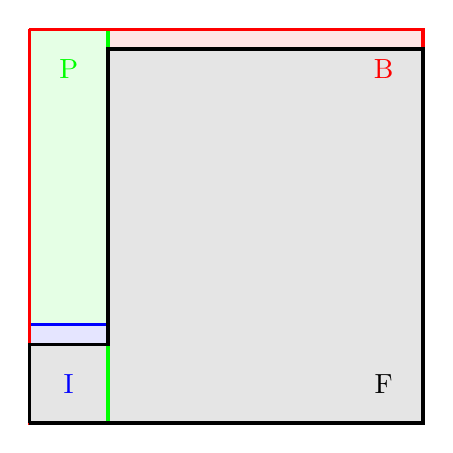
\begin{tikzpicture}[scale=0.5]
\fill[fill=red!10] (-5, 5) -- (5, 5) -- (5, -5) -- (-5, -5) -- (-5, 5);
\fill[green!10] (-5, 5) -- (-3, 5) -- (-3, -5) -- (-5, -5) -- (-5, 5);
\fill[blue!10] (-5, -2.5) -- (-3, -2.5) -- (-3, -5) -- (-5, -5) -- (-5, -2.5);
\fill[black!10] (-5, -5) -- (-5, -3) -- (-3, -3) -- (-3, 4.5) -- (5, 4.5) -- (5, -5) -- (-5, -5);
\draw[blue, very thick] (-5, -2.5) -- (-3, -2.5) -- (-3, -5) -- (-5, -5) -- (-5, -2.5);
\draw[green, very thick] (-5, 5) -- (-3, 5) -- (-3, -5) -- (-5, -5) -- (-5, 5);
\draw[red, very thick] (-5, 5) -- (5, 5) -- (5, -5) -- (-5, -5) -- (-5, 5);
\draw[black, very thick] (-5, -5) -- (-5, -3) -- (-3, -3) -- (-3, 4.5) -- (5, 4.5) -- (5, -5) -- (-5, -5);
\node[color=red] at (4, 4) {B};
\node[color=green] at (-4, 4) {P};
\node[color=blue] at (-4, -4) {I};
\node[color=black] at (4, -4) {F};
\end{tikzpicture}
\end{center}

\clearpage
\problem{}
From the definition of conditional probability, for $P(B) \neq 0$:
\begin{align*}
    P(A | B) = \frac{P(A, B)}{P(B)}
\end{align*}
Then:
\begin{align*}
    P(A | B) \cdot P(B) & = \frac{P(A, B)}{P(B)} \cdot P(B) \\
    P(A | B) \cdot P(B) & = P(A, B)
\end{align*}

\clearpage
\problem{}
Repeatedly applying the rule derived in Exercise 2:
\begin{align*}
    P(A, B, C, D) & = P(A | B, C, D) \cdot P(B, C, D) \\
    & = P(A | B, C, D) \cdot P(B | C, D) \cdot P(C, D) \\
    & = P(A | B, C, D) \cdot P(B | C, D) \cdot P(C | D) \cdot P(D)
\end{align*}

\clearpage
\problem{}
Let $E_0$ be the event that variable $X_i$ takes value $0$ and $E_1$ be the event that variable $X_i$ takes value $1$.
\begin{align*}
    E_0 & = \{x_i \in \Omega \mid x_i = 0\} \\
    E_1 & = \{x_i \in \Omega \mid x_i = 1\}
\end{align*}
Since $E_0$ and $E_1$ comprise the whole sample space ($E_0 \cup E_1 = \Omega$):
\begin{align*}
    P(E) = P((E \cap E_0) \cup (E \cap E_1))
\end{align*}
Then, since $E_0$ and $E_1$ are mutually disjoint ($E_0 \cap E_1 = \varnothing$):
\begin{align*}
    P(E) = P(E \cap E_0) + P(E \cap E_1)
\end{align*}
Using the definitions of $E_0$ and $E_1$:
\begin{align*}
    P(E) = \sum_{x \in E_0} P(E, X_i = x) + \sum_{x \in E_1} P(E, X_i = x)
\end{align*}
Since $x$ can only be in either $E_0$ or $E_1$:
\begin{align*}
    P(E) = \sum_{x} P(E, X_i = x)
\end{align*}

\clearpage
\problem{}
Repeatedly applying the rule derived in Exercise 4:
\begin{align*}
    P(X = 1, Y = 0) & = \sum_{u} P(X = 1, Y = 0, U = u) \\
    & = \sum_{u, v} P(X = 1, Y = 0, U = u, V = v) \\
    & = \sum_{u, v, w} P(X = 1, Y = 0, U = u, V = v, W = w)
\end{align*}

\clearpage
\problem{}
Suppose we have events $A$, $B$, and $C$ such that $P(B, C) \neq 0$ and $A$ and $B$ are independent given $C$. Then:
\begin{align*}
    P(A | B, C) & = \frac{P(A, B, C)}{P(B, C)} \\
    & = \frac{P(A, B | C) \cdot P(C)}{P(B, C)} \\
    & = \frac{P(A | C) \cdot P(B | C) \cdot P(C)}{P(B, C)} \\
    & = \frac{P(A | C) \cdot P(B, C)}{P(B, C)} \\
    & = P(A | C)
\end{align*}
\end{document}
